%% -*- encoding: utf-8 -*-
%% $Id$
\documentclass{clt2012}
\usepackage[utf8]{inputenc}
\usepackage{german}
\usepackage{amsmath,amsfonts,amsthm}
\usepackage{paralist}
\usepackage{fancyvrb}
\usepackage{listings}
\usepackage{tikz}
%\usepackage{eurosym}
\usepackage{lineno}
%\linenumbers
\renewcommand*\ttdefault{txtt}
\renewcommand{\figurename}{Bild}
\newcommand{\icofolder}{\includegraphics[width=1em]{icons/folder-bw}}
\newcommand{\icofiles}{\includegraphics[width=1em]{icons/page_white_stack-bw}}
\newcommand{\icofile}{\includegraphics[width=1em]{icons/page_white_text-bw}}
\lstset{basicstyle=\ttfamily,keywordstyle=\ttfamily\bfseries,breaklines,frame=single,xleftmargin=10pt}
\lstdefinestyle{numberedblock}{basicstyle=\ttfamily,keywordstyle=\ttfamily\bfseries,numbers=left,numberstyle=\scriptsize,xleftmargin=10pt,frame=single,breakindent=10pt}
\begin{document}
\title{Tic-\hspace{-0.2em}Tac-\hspace{-0.2em}Toe Reloaded --- Ein Mikrocontroller-Projekt mit Funkübertragung}
\author{Axel Wachtler, Jörg Wunsch, Matthias Vorwerk\\
\titleemail{\{axel,joerg,matthias\}@uracoli.de}\\
\titlewww{http://uracoli.nongnu.org/clt2012}}
\maketitle

\begin{abstract}
Das altbekannte Tic-Tac-Toe-Spiel wird in einem \mbox{ATmega128RFA1}-Mikro\-con\-trol\-ler\-pro\-jekt zu neuem Leben erweckt.
Es werden kapazitive und resistive Touch-Sensoren realisiert sowie eine drahtlose Datenübertragung in das Spiel integriert.
% Dabei werden zum einen kapazitive und resistive Touch-Sensoren und zum anderen
% drahtlose Übertragungstechnologien im Rahmen des Spiels realisiert.
Hierbei standen ein kostengünstiger und einfacher Aufbau der Hardware sowie eine leicht nachvollziehbare Software-Realisierung im Vordergrund.
\end{abstract}

\setlength{\parskip}{1ex}

%\tableofcontents
\section{Einführung}
Mikrocontroller sind mittlerweile Bestandteil verschiedenster Geräte des täglichen Lebens. Auf dem Markt existiert eine riesige Auswahl dieser interessanten Schaltkreise, angefangen von kleinsten 4-Bit-Varianten (z.\,B. in Fernbedienungen) über 8-Bit-Controller unterschiedlicher Größe und Komplexität (z.\,B. für Ladegeräte, Kühlschränke, Waschmaschinen) bis hin zu leistungsfähigen 32-Bit-Architekturen, die virtuelle Adressräume und Speicherverwaltung zur Verfügung stellen, sodass auf ihnen Mul\-ti\-task\-ing-Betriebssysteme laufen können.
Inzwischen sind Mikrocontroller mit integrierter Funkschnittstelle erhältlich. Damit können auch über längere Distanzen Informationen drahtlos übertragen werden. Ein Beispiel dafür ist der Controller \mbox{ATmega128RFA1} von Atmel. 

Das Ziel des Projektes ist es, eine Hardware zu entwickeln, die sowohl ein grundsätzliches
Verständnis der Beschaltung dieses interessanten Bauteils als auch den Aufbau und die
Funktionsweise der zum Betrieb nötigen Software vermittelt. Ansprechende 
Interaktionsmöglichkeiten für den Nutzer waren ebenso ausschlaggebend wie niedrige Hardwarekosten, die
durch ein minimalistisches Schaltungsdesign erreicht wurden.

Als Anwendungsbeispiel wird das jahrhundertealte Spiel \emph{Tic-Tac-Toe} ("`Drei gewinnt"') \cite{tictactoe} implementiert. 
Dabei spielen zwei Spieler auf einem 3x3-Spielfeld und belegen abwechselnd ein noch freies Feld mit einem eigenen
Symbol (z.\,B. Kreuz, Kreis). Ziel ist es, als erster eine komplette Zeile, Spalte oder Diagonale
mit dem eigenen Symbol zu belegen.
In der Mikrocontroller-Realisierung bedient jeder der beiden Spieler ein 3x3-Eingabefeld auf seiner eigenen Platine.
Als visuelle Rückmeldung werden jeweils 3x3-zweifarbige LED verwendet, die unter dem Eingabefeld aufleuchten.
Derjenige Spieler, welcher als erster eine Zeile, Spalte oder Hauptdiagonale mit "`seiner"' LED-Farbe belegt hat, gewinnt.
Die Spielereingaben werden über eine Funkverbindung zwischen beiden Platinen übertragen.

\section{Das Herzstück: Der ATmega128RFA1}

Als Mikrocontroller wird ein 8-Bit-AVR verwendet, da dieser Typ weit verbreitet ist und auch eine
hervorragende Unterstützung durch Open-Source-Entwicklungstools erfährt
(\texttt{avr-gcc}, \texttt{avr-libc}, \texttt{avr-gdb}, \texttt{avrdude}).
Der für dieses Projekt ausgewählte \mbox{ATmega128RFA1} \cite{atmega} ist ein 8-Bit-RISC-Controller
mit 128\,KiB Flash-Speicher, 4\,KiB EEPROM sowie 16\,KiB SRAM.
Er besitzt zusätzlich eine Funkschnittstelle nach dem \emph{IEEE-802.15.4}-Standard
für das 2,4-GHz-ISM-Band, mit der Daten mit 250\,kBit/s (Sondermodi bis zu 2\,MBit/s)
drahtlos übertragen werden können. Weiterhin enthält er einen 6 Bit breiten sowie vier
8 Bit breite Ein-/Ausgabeports, welche für die Ansteuerung der Leuchtdioden sowie der kapazitiven
und resistiven Sensorpads eingesetzt werden.
Weitere Einzelheiten zum Schaltkreis sind im Datenblatt \cite{atmega} nachzulesen.

\section{Verwendete Hardware}


\begin{figure}
\begin{minipage}[hbt]{0.45\linewidth}
	\centering
	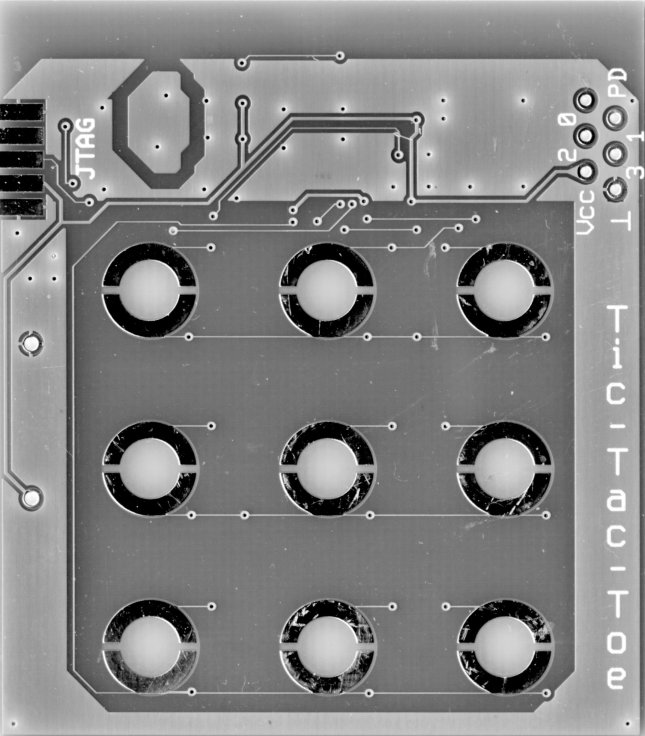
\includegraphics[width=\linewidth]{board_top}
	\caption{Leiterplattenoberseite mit resistiven Sensorflächen}
	\label{fig:board_top}
\end{minipage}
\hfill
\begin{minipage}[hbt]{0.45\linewidth}
	\centering
	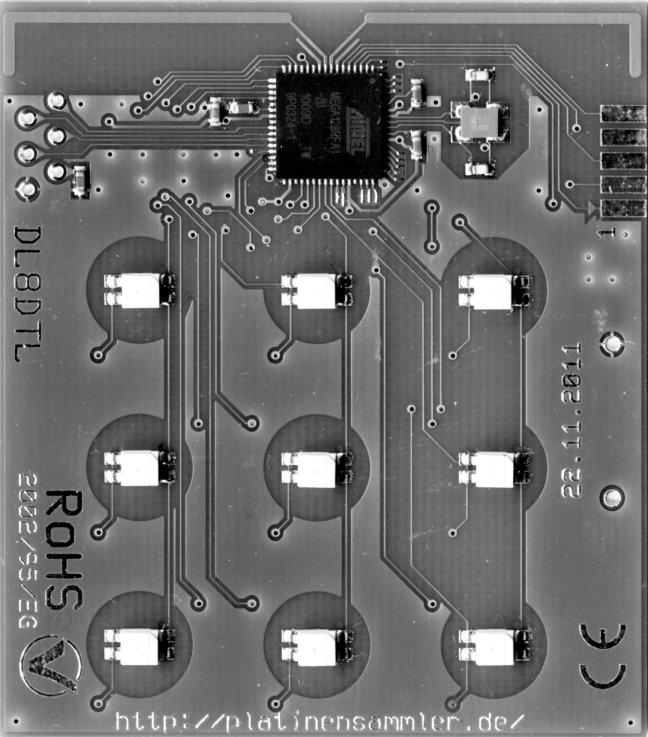
\includegraphics[width=\linewidth]{board_solder}
	\caption{Leiterplattenunterseite mit Mikrocontroller und LED}
	\label{fig:board_solder}
\end{minipage}
\end{figure}


Die Hardware besteht aus zwei eigens für diesen Zweck entwickelten, nahezu gleichen Platinen.
Jede Platine enthält:

\begin{itemize}
\setlength{\itemsep}{0pt}
\item einen AVR Mikrocontroller \mbox{ATmega128RFA1} mit \emph{IEEE-802.15.4}-Funk\-schnitt\-stel\-le von Atmel,
\item ein 3x3-Touchfeld aus Leiterzügen, wobei eine Platine aus resistiven und die zweite
      Platine aus kapazitiven Touch-Sensoren besteht,
\item 9 Zweifarb-LED, die ebenfalls als 3x3-Matrix auf der Unterseite
  der Platine angeordnet sind,
\item einen Batteriehalter,
\item einen 16-MHz-Quarz,
\item einige SMD-Kondensatoren,
\item verzinnte Anschlusspads für das JTAG-Programmierinterface,
\item Anschluss\-pads zu unbenutzten,
      digitalen Ein-/Ausgabepins (UART und $I^2C$-Interface) für eigene Erweiterungen.
\end{itemize}

Die gewählte Minimalbeschaltung zeigt zum einen, dass ein derartiger Mikrocontroller, abhängig
von den konkreten Anforderungen, mit sehr wenig Außenbeschaltung auskommen kann und erleichtert zum
anderen das Verständnis der Schaltung.

Durch die Verwendung von kapazitiven bzw. resistiven Sensoren konnten einerseits Drucktaster
eingespart werden, andererseits bietet dies die spannende Herausforderung, Algorithmen zur
zuverlässigen Erkennung von Fingerdrücken zu finden, was zusätzlichen
Softwareaufwand erfordert. Dieses Verlagern von Hardwareaufwand in die Software ist ein
durchaus üblicher und oft gewählter Ansatz.

\figurename{} \ref{fig:board_top} und \figurename{} \ref{fig:board_solder} zeigen
Platinenansichten. Die Sensorflächen befinden sich auf der Platinenoberseite.
Die LED auf der Bauteilseite durchscheinen die Leiterplatte und hinterleuchten so die Sensoren.

\section{Die Schaltung}

\begin{figure}[ht]
\centering % zum zentrieren, kannst Du auch weglassen
\fbox{
	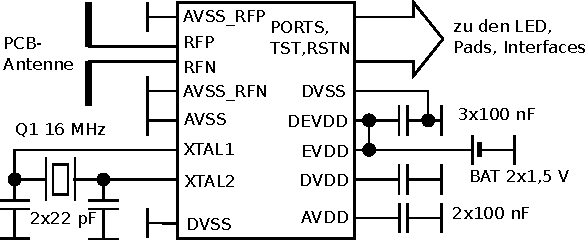
\includegraphics[width=0.6\linewidth]{uc_schem}
}
\caption{Außenbeschaltung des \mbox{ATmega128RFA1} (ohne LED/Touchmatrix)}
\label{fig:uc_schem}
\end{figure}


\begin{figure}[hbt]
\centering % zum zentrieren, kannst Du auch weglassen
\fbox{
	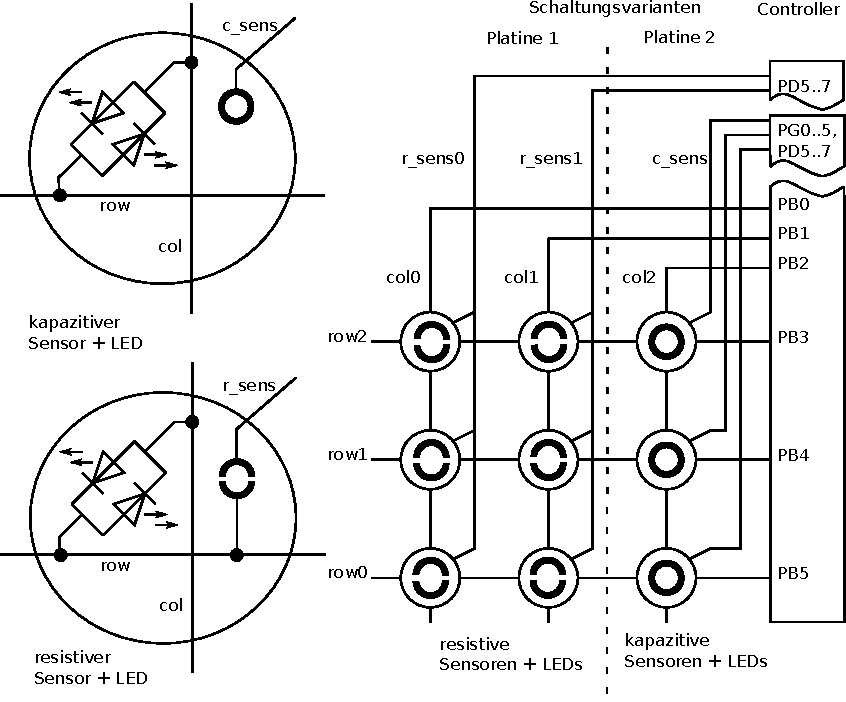
\includegraphics[width=0.95\linewidth]{matrix_schem_all}
}
\caption{Beschaltung der Ein-/Ausgabematrix für beide Platinenvarianten}
\label{fig:matrix}
\end{figure}

\figurename{} \ref{fig:uc_schem} zeigt die Beschaltung des Mikrocontrollers.
Neben einem 16-MHz-Quarz und zwei 22-pF-Lastkondensatoren, die mit der internen Oszillatorschaltung die notwendige stabile Frequenzreferenz für die Funkkommunikation liefern, sind lediglich noch fünf Stützkondensatoren für die Versorgungsspannung sowie neun Leuchtdioden zur Anzeige des Spielstandes als externe Bauelemente nötig.
Der Mikrocontroller selbst arbeitet mit einem 1-MHz-Takt, der durch einen internen RC-Oszillator mit nachgeschaltetem Teiler bereitgestellt wird.

Die Antenne wird als PCB-Antenne in Form von Leiterzügen auf der Platine realisiert. Auf das normalerweise in der
Grundbeschaltung vorgesehene Filter zur Unterdrückung unerwünschter Oberwellen an den HF-Pins wurde verzichtet.
Diese Vereinfachung erfüllt die Forderungen der Norm ETSI EN\,300\,440-1
(unerwünschte Aussendungen oberhalb 1\,GHz maximal 1\,$\mu$W) gerade noch
ausreichend; zur Erhöhung des Sicherheitsabstandes ist ein Betrieb mit
leicht reduzierter Sendeleistung (-5\,dBm) ratsam.  Ein Betrieb außerhalb
des Geltungsbereiches der europäisch harmonisierten Regelungen ist jedoch
mit dieser einfachen Anordnung in der Regel nicht zulässig.


Die Schaltung der LED- und Sensormatrix für beide Platinenvarianten ist in \figurename{} \ref{fig:matrix} dargestellt.
Die Pins 3, 4, 5 von Port B bilden die drei Zeilenleitungen, die Pins 0, 1, 2 die Spaltenleitungen der 3x3-LED-Matrix. Die Leuchtdiodenmodule befinden sich an den Kreuzungspunkten der Zeilen- und Spaltenleitungen. Durch High/Low-Ausgaben an den entsprechenden Bits dieses Ports kann jeweils eine der beiden antiparallel geschalteten unterschiedlich farbigen Leuchtdioden eingeschaltet werden. Aufgrund des geringen maximalen Stroms der Ausgangstreiber im Schaltkreis ist es möglich, auf die ansonsten notwendigen Vorwiderstände zu verzichten. 

Für die Touch-Sensoren wurden zwei unterschiedliche Ansätze gewählt, um die Work\-shop-Teil\-nehmer mit verschiedenen Realisierungsvarianten für ein gegebenes Problem bekannt zu machen.
% Zudem bleibt hierdurch viel Raum für eigene Experimente.

Die kapazitiven Sensoren wurden als Leiterzüge in Form von breitrandigen Kreisen realisiert, um einerseits eine möglichst große
Kapazitätsfläche zu erreichen und andererseits ein Durchscheinen der auf der Gegenseite angeordneten LED zu gewährleisten.
Alle neun Sensorflächen werden separat an die Pins 5, 6, 7 (Port D) und 0 -- 5 (Port G) geführt.

Im Gegensatz zu den kapazitiven Sensoren werden für den resistiven Ansatz zwei Leitungen pro Sensor benötigt.
Um das Platinendesign einfach zu  halten und die Zahl der notwendigen Ein-/Ausgabeports zu beschränken, 
werden die 3x3-Sensoren ebenfalls matrixförmig durch Zeilen- und Spaltenleitungen angesteuert,
wobei die Sensoren an den Kreuzungspunkten angeordnet sind. Als Zeilenleitungen werden die für
die LED-Ansteuerung verwendeten Leitungen mit genutzt (Pins 3, 4, 5 von Port B); die Spaltenleitungen
werden mit den Pins 5, 6, 7 von Port D verbunden.

Die kompletten Schaltungsunterlagen sind auf der Projektwebseite zu finden.

\subsection*{Die kapazitiven Touch-Sensoren}

Die Wirkungsweise der kapazitiven Sensoren wird in \figurename{} \ref{fig:capsense} gezeigt. Vor Beginn eines Abfragevorgangs
($t < t_0$) ist der Schalter $S_d$ geschlossen. Die Kapazität $C_{in}=C_{pin} + C_{pad}$, die sämtliche gegen Masse wirkenden Kapazitäten zusammenfasst, ist entladen, und an der Leitung \texttt{c\_sens} liegt eine Spannung von 0 Volt an.

\begin{figure}[hb]
\centering
\fbox{
	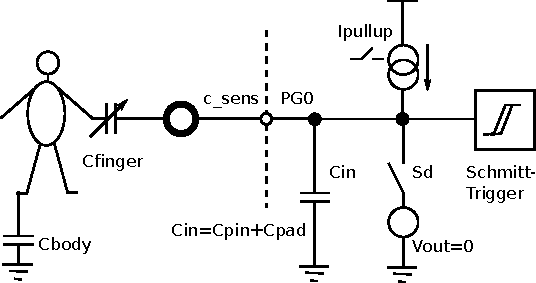
\includegraphics[scale=0.7]{cap_sense}
}
\caption{Wirkungsprinzip kapazitiver Sensor}
\label{fig:capsense}
\end{figure}

Zu Beginn der Messung bei $t = t_0$ wird $S_d$ geöffnet (Abschalten des Ausgangstreibers) und ein Pullup-Strom
$I_{pullup}$ beginnt, die Kapazität aufzuladen. Wegen $I = C du/dt$ ist der messbare Spannungsanstieg je Zeiteinheit am Pin durch die Kapazität bestimmt. Die Zeit $t'-t_0$ bis zum Schalten des Schmitt-Triggers ist somit ein Maß für die Gesamtkapazität am Pin.

Bei Berührung des Sensors wird eine weitere Kapazität  $\cfrac{1}{(1/C_{finger} + 1/C_{body})}$ parallel zu $C_{in}$ 
wirksam, was in einer längeren Aufladezeitdauer $t''-t_0$ resultiert. Für die Erkennung einer Berührung wird in der Software eine Zeit $t_{sample}$ mit $t' < t_{sample} < t''$ als Entscheidungskriterium genutzt.

Entscheidend für die sichere Erkennung einer Berührung des Sensors ist $t'' \gg t'$ und somit eine möglichst große Kapazitätsänderung. 

$C_{body}$ ist wegen $C \sim A/d$ aufgrund der Körperoberfläche hinreichend groß. Eine hohe Kapazität $C_{finger}$ wird erreicht,
indem der direkt auf auf die Kapazitätsflächen aufgebrachte Lötstopplack mit einer Dicke von wenigen 10 $\mu$m ein sehr dünnes Dielektrikum zwischen Finger und Sensorfläche bildet. Durch diese Anordnung kann die gewünschte hohe Kapazitätsänderung erreicht werden.

Es ist zu beachten, dass $I_{pullup}$ stark betriebsspannungsabhängig ist (5 \dots 30 $\mu$A). Wegen $du/dt = I_{pullup}/C_{total}$ muss die relative Kapazitätsänderung im Berührungsfall deutlich größer als die zu erwartende relative Variation des Pullup-Stroms sein,
um dennoch eine sichere Berührungserkennung gewährleisten zu können. 
Gegebenenfalls sind Kalibriermessungen denkbar, die eine Anpassung von $t_{sample}$ in Abhängigkeit der gemessenen Versorgungsspannung $V_{cc}$ und der Zeit $t'$ zur Folge haben. Für die derzeitige Software-Realisierung ist dies nicht vorgesehen.

\subsection*{Die resistiven Touch-Sensoren}

Das Funktionsprinzip der resistiven Sensoren ist in \figurename{} \ref{fig:ressense} dargestellt. 

Die beiden Sensorkontakte werden durch den symbolischen Widerstand $R_{finger}$ nachgebildet. Dessen Widerstandswert kann,
wenn beide Kontakte durch einen Finger berührt werden, abhängig von mehreren Faktoren (Hautfeuchte, Druckstärke, \dots)
stark variieren und liegt zum Teil im zweistelligen Megaohm-Bereich. In der Kapazität $C_{in}=C_{pin} + C_{pad}$ werden
alle parasitären Eingangskapazitäten der Leitung \texttt{r\_sens} zusammengefasst. Eine weitere parasitäre Kapazität
$C_{par}$ parallel zu den beiden Sensorkontakten bildet mit $C_{in}$ einen kapazitiven
Spannungsteiler. Da $C_{par} \ll  C_{in}$ gilt, wird im Einschaltmoment $t=t_0$ die
Schaltschwelle des Triggers nicht erreicht. Im folgenden wird $C_{par}$ nicht weiter betrachtet.

\begin{figure}[hbt]
\centering
\fbox{
	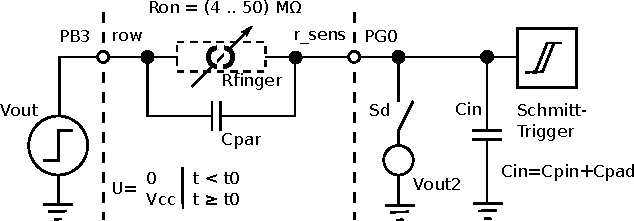
\includegraphics[scale=0.7]{res_sense}
}
\caption{Wirkungsprinzip resistiver Sensor}
\label{fig:ressense}
\end{figure}

Vor Beginn der Messung bei $t < t_0$ beträgt die Ausgangsspannung des treibenden Ausgangspins (Leitung \texttt{row}) 0 Volt. Die
Leitung \texttt{r\_sens} ist ebenfalls als Ausgang und auf 0 Volt geschaltet ($S_d$ geschlossen). $C_{par}$ und $C_{pin} + C_{pad}$ sind entladen.

Zu Beginn der Messung ($t = t_0$) wird $S_d$ geöffnet und das Sense-Pin (PG0 in \figurename{} \ref{fig:ressense}) wird als Eingang betrieben. Gleichzeitig wird die
Zeilenleitung \texttt{row} auf $V_{cc}$ geschaltet (Ausgangspegel High). In Abhängigkeit von $R_{finger}$ wird nun $C_{in}$
auf die Spannung $U(t-t_0) = V_{cc} (1 - e^{-(t-t_0)/\tau})$ mit $\tau = R_{finger} C_{in}$ aufgeladen.
Bei Erreichen der Schaltschwelle des Schmitt-Triggers nach der Zeit $t'-t_0$ schaltet das entsprechende Eingangsbit auf 1.

Für angenommene Werte $R_{finger}=50\,$M$\Omega$ und $C_{in} \approx 20$\,pF wird die Schaltschwelle 
$V_{cc}/2$ nach $t'-t_0=\tau \ln 2 = 0,69$\,ms erreicht. Für $R_{finger}=1\,$M$\Omega$ (minimaler Überbrückungswiderstand durch den
Finger) ergibt sich eine Zeit von $t'-t_0=13,86\,u$s. Eine sichere Erkennung erfordert mithin u.\,U. eine relativ lange Messzeit.


\section{Software-Realisierung}

Die Software wird in der Programmiersprache C geschrieben.
Ein wichtiger Bestandteil sind die Routinen zur
Abfrage der Touch-Sensoren. Die zeitlich exakte Messung der kurzen
Aufladezeit der kapazitiven Sensoren wird durch 16-faches sequenzielles
Einlesen der Input-Port-Information realisiert und erfordert die Verwendung von
Inline-Assembler-Code.

Da die Leuchtdioden matrixförmig verschaltet sind, ist eine zeilenweise,
zeitmultiplexe Ansteuerung notwendig. Diese und die zyklische Abfrage
der Berührungssensoren werden in einer Interruptroutine ausgeführt, die per
Timer gestartet wird.

% \subsection*{Die $\mu{}$racoli Library}

Die Datenübertragung zwischen den beiden Knoten erfolgt über die eingebaute Funk\-schnitt\-stel\-le des
\mbox{ATmega128RFA1}, um beiden Spielern den aktuellen Spielstand synchron anzeigen zu können.
Die Ansteuerung der integrierten Sende- und Empfangsbaugruppen erfordert prinzipiell einen nicht unerheblichen
Softwareaufwand, der den Rahmen dieses Projektes bei Weitem sprengen würde.\newline
Mit dem \textbf{$\mu{}$racoli-Projekt} \cite{uracoli} existiert für
diesen und verwandte Schaltkreise von Atmel eine freie Softwarebibliothek, die die
Low-Level-Ansteuerung der Funkbaugruppen
dieser Schaltkreise übernimmt und High-Level-Funktionen \texttt{radio\_send\_frame()} und
\texttt{usr\_radio\_receive\_frame()} zur Übertragung kompletter Datensätze zur Verfügung stellt.

Die vollständige Software zu diesem Projekt steht unter einer modifizierten BSD-Lizenz
und ist auf der zugehörigen Webseite \cite{uracoli} zu finden.

\section{Übersetzen und Inbetriebnahme}

Zum Entwickeln, Übersetzen und Programmieren der Controller wurde die 
\emph{AVR}-Toolchain für Linux verwendet, bestehend aus dem GCC-Compiler \texttt{avr-gcc}, dem Linker aus den
\emph{GNU binutils} und der \texttt{avr-libc}. Der Programmieradapter wird mit dem Programm \texttt{avrdude} angesteuert.
Beispiele für integrierte Entwicklungsumgebungen, die ebenso genutzt werden können (und dann teilweise oder vollständig auf der genannten Toolchain aufsetzen), sind das
\emph{AVR Studio} \cite{avrstudio} (nur für Windows), \emph{Eclipse} oder \emph{Code::Blocks}.

Zur Programmierung der Mikrocontroller können die \emph{AVR-Dragon}-Boards von Atmel zum Einsatz kommen.
Deren mitgeliefertes Kabel wird mit einem Zwischenadapter verbunden, welcher direkt auf die vorgesehenen
verzinnten JTAG-Anschluss\-fahnen der Platinen gesteckt wird.

Neben der Programmierung ist es auch möglich, über das JTAG-Interface \emph{On Chip Debugging}
durchzuführen. Hierzu stellt das Tool \texttt{avarice} eine Verbindung zwischen dem Schaltkreis und
dem \texttt{avr-gdb} (Debugger) her, sodass schrittweise Prog\-ramm\-ab\-ar\-beitung und die Abfrage interner
Register möglich ist. 

\section{Ausblick}

Die entwickelten Platinen ermöglichen es, erste Hardware- und Programmiererfahrungen mit
AVR-Mikrocontrollern zu sammeln.
Da die Platinen neben neun zweifarbigen LED und neun Eingabefeldern auch die Möglichkeit der
Funkkommunikation nach dem \emph{IEEE-802.15.4}-Standard bieten, sind eine Vielzahl anderer
Einsatzmöglichkeiten denkbar. Die realisierte Version des Tic-Tac-Toe-Spiels soll lediglich als Anregung dienen und Lust auf eigene Experimente machen.
Über Anregungen, Fragen und aktive Hilfe freut sich das $\mu{}$racoli-Team.


\begin{thebibliography}{XX}
\bibitem{uracoli}
    \emph{$\mu{}$racoli - The Micro Controller Radio Communication Library}. Homepage\\
    \url{http://uracoli.nongnu.org}
\bibitem{tictactoe}
	\emph{Tic Tac Toe}. Wikipedia\\
	\url{http://de.wikipedia.org/wiki/Tic_Tac_Toe}
\bibitem{atmega}
	\emph{ATmega128RFA1} Herstellerinformationen\\
	\url{http://www.atmel.com/dyn/products/product_card.asp?part_id=4692}
\bibitem{avrstudio}
	\emph{Atmel AVR Studio}. Produktseite\\
	\url{http://www.atmel.com/avrstudio}
\bibitem{drahtlosesensoren}
	A. Wachtler, J. Wunsch, M. Vorwerk, \emph{Drahtlose Sensordatenerfassung und -ver\-arbeitung mit Linux}. 
    Tagungsband Chemnitzer Linuxtage 2011. Chemnitz 2011. 13-20
\end{thebibliography}
\end{document}
